\section{A Generalized Version of Dynamic KAC}
\label{sec:general}

In this section, we focus on building an efficiently extensible version of our proposed scheme that allows an user to economically increase the number of ciphertext classes while registering a new public key-private key pair. We adopt the idea presented in \cite{boneh2005collusion} to develop a hierarchical structure that has multiple instances (say $n_1$) of the original scheme running in parallel. Each such instance in turn provides \emph{locally aggregate keys} for $n_2$ ciphertext sub-classes. Each ciphertext class thus now has a double index $(i_1,i_2)$ where $1\leq i_1 \leq n_1$ and $1\leq i_2 \leq n_2$. This allows the overall setup to handle $n=n_1n_2$ classes. However, it is important to note that all the instances can use the same public parameters. This interaction among the instances helps to largely improve performance. We further point out that while in \cite{boneh2005collusion}, the generalized construction offers a trade-off between the public parameter size and the ciphertext size, our 
generalized scheme actually reduces the public parameter size without compromising on the size of the ciphertext. Further, addition of a single new key increases the number of classes only by $n_2$ and not by $n$. Setting $n_2\ll n$ thus achieves significant improvement in performance over the existing proposal.


\subsection{The Construction of the Generalized KAC}
\label{subsec:construction2}

Let $n_2$ be a fixed positive integer. Our proposed $n_2$-generalized key-aggregate encryption scheme over elliptic curve subgroups is as described below. It may be noted that the bilinear additive elliptic curve sub-group $\mathbb{G}$ and the multiplicative group $\mathbb{G}_T$, as well as the pairing $\hat{e'}$ are the same as in the basic scheme. The algorithm sets up $n_1=\lfloor n/n_2\rfloor$ instances of the basic scheme, each of which handles $n_2$ ciphertext classes. The original scheme is thus a special case of the extended scheme with $n_1=1$ and $n_2=n$.


\begin{enumerate}
 \item \textbf{Setup}$(1^{\lambda},n_2)$: Randomly pick $\alpha \in \mathbb{Z}_q$. Compute $P_i$ = ${\alpha^{i}}P \in \mathbb{G}$ for $i = 1,\cdots,n_2,n_2+2,\cdots,2n_2$. Output the system parameter as\\
 $param$ = $(P,P_1,\cdots,P_{n_2},P_{n_2+2},\cdots,P_{2n_2})$. The system randomly chooses a secret parameter $t \in \mathbb{Z}_q$ which is not made public. It is only known to data owners with credentials to control client access rights.
 \item \textbf{Keygen}(): Pick $\gamma_1,\gamma_2,\cdots,\gamma_{n_1} \in \mathbb{Z}_q$, output the public and master-secret key pair :\\ $(PK$=$({pk}_1,pk_{2},\cdots,pk_{n_1})=(\gamma_1P,\gamma_2P,\cdots,\gamma_{n_1}P)$,$msk$=$(\gamma_1,\gamma_2,\cdots,\gamma_{n_1}))$.
 \item \textbf{Encrypt}$(pk_{i_1},(i_1,i_2),m)$: For a message $m \in \mathbb{G}_T$ and an index $(i_1,i_2) \in \{1,2,\cdots,n_1\}\times\{1,2,\cdots,n_2\}$, randomly choose $r\in\mathbb{Z}_q$ and let $t'=t+r \in\mathbb{Z}_q$. Then compute the ciphertext $\mathcal{C}$=$(rP,t'{(pk_{i_1}+P_{i_2})},m.\hat{e'}(P_{n_2},t'P_1))$ = $(c_1,c_2,c_3)$.
 \item \textbf{Extract}$(msk=\gamma,\mathcal{S})$: For the set $\mathcal{S}$ of indices $(j_1,j_2)$ the aggregate key is computed as $K_{\mathcal{S}}$ = $(k^{1}_{\mathcal{S}},k^{2}_{\mathcal{S}},\cdots,k^{n_1}_{\mathcal{S}})$ =\\$(\sum_{(1,j_2)\in\mathcal{S}}{\gamma_{1}}P_{n_2+1-j_2},\sum_{(2,j_2)\in\mathcal{S}}{\gamma_{2}}P_{n_2+1-j_2},\cdots,\sum_{(n_1,j_2)\in\mathcal{S}}{\gamma_{n_1}}P_{n_2+1-j_2})$\\ and the dynamic access control parameter $U$ is computed as $tP$. Thus the net aggregate key is $(K_{\mathcal{S}},U)$ which is transmitted via a secure channel to users that have access rights to $\mathcal{S}$. Note that  $k^{j_1}_{\mathcal{S}}=\sum_{(j_1,j_2)\in\mathcal{S}}\alpha^{n+1-j_2}pk_{j_1}$ for $j_1=1,2,\cdots,n_1$. 
 \item \textbf{Decrypt}$(K_{\mathcal{S}}, U, \mathcal{S},(i_1,i_2),\mathcal{C}=\{c_1,c_2,c_3\})$: If $(i_1,i_2)\notin\mathcal{S}$, output $\bot$. Otherwise return the message\\ $\hat{m}$ = $c_3\frac{\hat{e'}(k^{i_1}_{\mathcal{S}}+\sum_{(i_1,j_2)\in\mathcal{S},j_2\neq i_2}P_{n_2+1-j_2+i_2},U+c_1)}{\hat{e'}(\sum_{(i_1,j_2)\in\mathcal{S}}P_{n_2+1-j_2},c_2)}$. 
\end{enumerate}

The proof of correctness for the generalized scheme is very similar to that for the basic scheme.

\subsection{Semantic Security of the Generalized KAC}
\label{subsec:proof_general}

\subsubsection{The Reduced Generalized Scheme:}

We define a reduced version of the generalized encryption scheme. We note that the ciphertext $\mathcal{C}=(c_1,c_2,c_3)$ output by the $Encypt$ operation essentially embeds the value of $m$ in $c_3$ by multiplying it with $\hat{e'}(P_{n_2},tP_1)$. Consequently, the security of our proposed scheme is equivalent to that of a \emph{reduced} generalized key-aggregate encryption scheme that simply uses the reduced ciphertext $(c_1,c_2)$, the aggregate key $K_{\mathcal{S}}$ and the dynamic access parameter $U$ to successfully transmit and decrypt the value of $\hat{e'}(P_{n_2},t'P_1)=\hat{e'}(P_{n_2+1},t'P)$. We prove the semantic security of this \emph{reduced scheme} parameterized with a given number of ciphertext classes $n_2$ for each instance, which also amounts to proving the semantic security of our original encryption scheme for the same number of ciphertext classes. Note that the proof of security is independent of the number of instances $n_1$ that run in parallel.

\subsubsection{The Adversarial Model:} We make the following assumptions about the adversary $\mathcal{A}$:

\begin{enumerate}
 \item The adversary has the aggregate key that allows her to access any ciphertext class other than those in the target subset $\mathcal{S}$, that is, she possesses $K_{\overline{\mathcal{S}}}$.
 \item The adversary has access to the public parameters $param$ and $PK$, and also possesses the dynamic access parameter $U$.
%  \item The adversary is authorized and and hence 
\end{enumerate}


\subsubsection{The Security Proof:}

The security proof presented here uses the first complexity assumption stated in \ref{subsubsec:asm_1}. Let $\mathbb{G}$ be a bilinear elliptic curve subgroup of prime order $q$ and $G_T$ be a multiplicative group of order $q$. Let $\hat{e'}:\mathbb{G} \times \mathbb{G}\longrightarrow\mathbb{G}_T$ be a bilinear non-degenerate pairing. For any pair of positive integers $n_2,n' (n'>n_2)$ our proposed $n_2$-generalized reduced key-aggregate encryption scheme over elliptic curve subgroups is $(\tau,\epsilon,n')$ semantically secure if the decision $(\tau,\epsilon,n_2)$-BDHE assumption holds in $\mathbb{G}$. We now prove this statement below.

\textbf{\noindent{Proof:}} Let for a given input $n'$, $\mathcal{A}$ be a $\tau$-time adversary that has advantage greater than $\epsilon$ for the \emph{reduced scheme} parameterized with a given $n_2$. We build an algorithm $\mathcal{B}$ that has advantage at least $\epsilon$ in solving the $n_2$-BDHE problem in $\mathbb{G}$. Algorithm $\mathcal{B}$ takes as input a random $n_2$-BDHE challenge $(P,H,Y_{(P,\alpha,n_2)},Z)$ where $Z$ is either $\hat{e'}(P_{n_2+1},H)$ or a random value in $\mathbb{G}_T$. Algorithm $\mathcal{B}$ proceeds as follows.

\begin{enumerate}
 \item \textbf{Init:} Algorithm $\mathcal{B}$ runs $\mathcal{A}$ and receives the set $\mathcal{S}$ of ciphertext classes that $\mathcal{A}$ wishes to be challenged on. For each ciphertext class $(i_1,i_2)\in\mathcal{S}$, $\mathcal{B}$ performs the \textbf{SetUp}-$\mathbf{(i_1,i_2)}$, \textbf{Challenge}-$\mathbf{(i_1,i_2)}$ and \textbf{Guess}-$\mathbf{(i_1,i_2)}$ steps. Note that the number of iterations is polynomial in $|S|$. 
 
 \item \textbf{SetUp}-$\mathbf{(i_1,i_2)}$: $\mathcal{B}$ should generate the public $param$, public key $PK$, the access parameter $U$, and the aggregate key $K_{\overline{\mathcal{S}}}$. For the iteration corresponding to ciphertext class $(i_1,i_2)$, they are generated as follows.
 \begin{itemize}
  \item $param$ is set as $(P,Y_{P,\alpha,n_2})$.
  \item Randomly generate $u_1,u_2,\cdots,u_{n_1} \in \mathbb{Z}_q$. Then, set $PK$=\\$(pk_1,pk_2,\cdots,pk_{n_1})$, with $pk_{j_1}$ = $u_{j_1}P - P_{i_2}$ for $j_1=1,2,\cdots,n_1$.
  \item Set $K_{\overline{\mathcal{S}}}$ = $(k^{1}_{\overline{\mathcal{S}}},k^{2}_{\overline{\mathcal{S}}},\cdots,k^{n_1}_{\overline{\mathcal{S}}})$, where $k^{j_1}_{\overline{\mathcal{S}}}$ is set as $\sum_{(j_1,j_2)\notin\mathcal{S}}({u_{j_1}}P_{n_2+1-j_2}-(P_{n_2+1-j_2+i_2}))$. Then, $k^{j_1}_{\overline{\mathcal{S}}}$ = $\sum_{(j_1,j_2)\notin\mathcal{S}}\alpha^{n_2+1-j_2}pk_{j_1}$,which is as per the scheme specification. Note that $\mathcal{B}$ knows that $(i_1,i_2)\notin \overline{\mathcal{S}}$, and hence has all the resources to compute this aggregate key for $\overline{\mathcal{S}}$. 
  \item $U$ is set as some random element in $\mathbb{G}$.
 \end{itemize}
 
 Note that since $P$, $\alpha$, $U$ and the $u_{j_1}$ values are chosen uniformly at random, the public key has an identical distribution to that in the actual construction.
 
 \item \textbf{Challenge}-$\mathbf{(i_1,i_2)}$: To generate the challenge for the ciphertext class $(i_1,i_2)$, $\mathcal{B}$ computes $(c_1,c_2)$ as $(H-U,u_{i_1}H)$. It then randomly chooses a bit $b\in{(0,1)}$ and sets $K_b$ as $Z$ and $K_{1-b}$ as a random element in $\mathbb{G}_T$. The challenge given to $\mathcal{A}$ is $((c_1,c_2),K_0,K_1)$. 
 
 We claim that when $Z=\hat{e'}(P_{n_2+1},H)$ (i.e. the input to $\mathcal{B}$ is a $n_2$-BDHE tuple), then $((c_1,c_2),K_0,K_1)$ is a valid challenge to $A$. We prove this claim here. we point out that $P$ is a generator of $\mathbb{G}$ and so $H=t'P$ for some $t'\in\mathbb{Z}_q$. Putting $H$ as $t'P$ gives us the following:
 \begin{itemize}
  \item  $U=tP$ for some $t\in\mathbb{Z}_q$
  \item $c_1=H-U=(t'-t)P=rP$ for $r=t'-t$
  \item $c_2=u_{i_1}H=(u_{i_1})t'P=t'(u_{i_1}P)=t'(u_{i_1}P-P_{i_2}+P_{i_2})=t'(pk_{i_1}+P_{i_2})$
  \item $K_b=Z=\hat{e'}(P_{n_2+1},H)=\hat{e'}(P_{n_2+1},t'P)$
 \end{itemize}
 On the other hand, if $Z$ is a random element in $\mathbb{G}_T$ (i.e. the input to $\mathcal{B}$ is a random tuple), then $K_0$ and $K_1$ are just random independent elements of $\mathbb{G}_T$.
 
 \item\textbf{Guess}-$\mathbf{(i_1,i_2)}$: The adversary $\mathcal{A}$ outputs a guess $b'$ of $b$. If $b' = b$, $\mathcal{B}$ outputs $0$ (indicating that $Z = \hat{e'}(P_{n_2+1},H)$), and terminates. Otherwise, it goes for the next ciphertext class in $\mathcal{S}$.
\end{enumerate}
If after $|\mathcal{S}|$ iterations, $b' \neq b$ for each ciphertext class $(i_1,i_2)\in\mathcal{S}$, the algorithm $\mathcal{B}$ outputs $1$ (indicating that $Z$ is random in $\mathbb{G}_T$). We now analyze the probability that $\mathcal{B}$ gives a correct output. If $(P,H,Y_{(P,\alpha,n_2)},Z)$ is sampled from $R$-BDHE, $Pr[\mathcal{B}(G,H,Y_{(P,\alpha,n_2)},Z)=0]$ = $\frac{1}{2}$, while if $(P,H,Y_{(P,\alpha,n_2)},Z)$ is sampled from $L$-BDHE, $|Pr[\mathcal{B}(G,H,Y_{(P,\alpha,n_2)},Z)]-\frac{1}{2}|$ $\geq$ $\epsilon$. So, the probability that $\mathcal{B}$ outputs correctly is at least $1-(\frac{1}{2}-\epsilon)^{|\mathcal{S}|} \geq \frac{1}{2}+\epsilon$. Thus $\mathcal{B}$ has advantage at least $\epsilon$ in solving the $n_2$-BDHE problem. This concludes the proof. \emph{Note that the instance of this proof with $n_1=1$ and $n_2=n$ serves as the proof of security for the basic KAC scheme proposed in Section \ref{sec:proposal}}.


\subsubsection{Performance Trade off with the Basic Scheme:} 

We compare the various parameter sizes for the proposed original and extended schemes in table \ref{tab:tradeoff}. We note that $SetUp$ and $KeyGen$ are both one-time operations, and for a given subset $\mathcal{S}$, the $Extract$ operation is also performed once to generate the corresponding aggregate key $K_{\mathcal{S}}$. The most important advantage that the generalized scheme provides is the user's ability to efficiently extend the number of ciphertext classes. As far as encryption and decryption are concerned, encryption should ideally take the same time for both schemes, while decryption is actually expected to be faster for the generalized construction as $n_2\leq n$.  

\begin{table}[!t]
\captionsetup{font=scriptsize}
\caption{Comparison between the Basic and Generalized schemes}
\label{tab:tradeoff}
\begin{center}
\scalebox{0.75}{
\begin{tabular}{|c|c|c|c|}

%Symbol & Fault Model \\
%(MHz)&$\ $ &$\ $ & $\ $\\
\hline
\textbf{Item} & \textbf{Nature of Computation} & \textbf{Original scheme} & \textbf{Generalized scheme}\\\hline\hline

$param$(SetUp) & One-time & $\mathcal{O}(n)$ & $\mathcal{O}(n_2)$\\\hline
$PK$(KeyGen) & One-time &$\mathcal{O}(1)$ & $\mathcal{O}(n_1)$\\\hline
$K_{\mathcal{S}}$(Extract) & One-time & $\mathcal{O}(1)$ & $\mathcal{O}(n_1)$\\\hline
$\mathcal{C}$ & One per Message & $\mathcal{O}(1)$ & $\mathcal{O}(1)$\\\hline
Encrypt & One Per Message & $\mathcal{O}(1)$ & $\mathcal{O}(1)$\\\hline
Decrypt & One Per Message & $\mathcal{O}(|\mathcal{S}|)$ & $\mathcal{O}(|\mathcal{S}|)$\\\hline
% Ciphertext Class Extension & Dynamic & Not Possible & $\mathcal{O}(n_2)$\\\hline
\hline
% OSB & Other Single Byte Faults (More than 4 bits in one byte affected)  \\
% MB & Multiple Byte Faults  \\

% \hline \hline
\end{tabular}
}

\end{center}
\end{table}


\subsection{A Flexible Extension Policy}
\label{subsec:extension}

If a user needs to classify her ciphertexts into more that $n$ classes, she can register for additional key pairs $(pk_{n_1+1},msk_{n_1+1})$, $\cdots$, $(pk_{n_1+l},msk_{n_1+l})$ as per her requirements. Each new key registration increases the number of classes by $n_2$, where $n_2\leq n$. The idea of under-utilization stems from the fact that registration of each public-private key pair increases the number of classes by $n_2$. However, it is not necessary that all the existing classes are utilized at any given point of time. For instance, a user may at any point of time want to register $l$ new private-public key pairs, however she will in all probability not use up all $ln_2$ additional classes of messages that could be encrypted using the newly registered keys. We stress here is that, unlike in the public key extension scheme proposed in \cite{chu2014key} where the values of $n_1$ and $n_2$ are fixed to $1$ and $n$ respectively, our generalized construction \emph{provides a choice} of $n_1$ and $n_2$ so that the system administrator could choose pair of values suited to their requirements. 

We propose a metric to quantify the under-utilization of ciphertext classes for a given configuration of the system. Let us assume that at some instance of time, there are $n_1+l$ private-public key pairs registered in the system, and $c_i$ classes corresponding to each key are being utilized. We define the utilization coefficient as $\frac{1}{1+\xi}$, where $\xi=-\frac{1}{n_1}\sum_{i=1\\c_i\neq0}^{n_1}\log(\frac{c_i}{n_2})$. An efficient scheme tries to minimize the value of $\xi$ to achieve good utilization of the existing set of classes. The value is maximum when $c_i=n_2 \forall i=1,2,\cdots,n_2$. Note that $c_i=0$ implies that no subclasses under the given key $pk_i$ are being utilized, which is equivalent to not registering the key at all.        


To stress the importance of the flexible extension policy, we provide a simplified example here. We consider two possible configurations of the extended scheme. In the first configuration, $n_1=1$ and $n_2=n$, which is essentially identical to the public key extension scheme proposed in \cite{chu2014key}. The other configuration has $n_1>1$ and $n_2<n$. Now assume that before extension, both schemes utilized $c$ ciphertext classes out of the $n$ possible classes, equally distributed across all key pairs. Now suppose a situation arises where an user needs to register $l$ more key pairs, and utilizes $z<n_2$ classes corresponding to each key. In the first configuration, we have $\xi_1=-\frac{1}{l+1}(l\log(\frac{z}{n})+\log(\frac{c}{n}))$, while for the second configuration, $\xi_2=-\frac{1}{l+n_1}(l(\log(\frac{z}{n_2}))+n_1\log(\frac{c}{n}))$. Now for $l>(\frac{n_1}{\log n_1}-1)\log(\frac{z}{c})-1$, $\xi_2<\xi_1$. Thus for any value of $(n_1,n_2)$ other than $(1,n)$, there exists a value of $l$ for which the 
scheme achieves better utilization coefficient. Since $l$ is expected to increase in a dynamic scenario, our public key extension scheme eventually performs better than the scheme suggested in \cite{chu2014key}. 

\subsection{Advantage over Hierarchical Encryption Based Schemes}
\label{subsec:advantage}

\begin{figure}[!t]
\centering
\captionsetup{font=scriptsize}
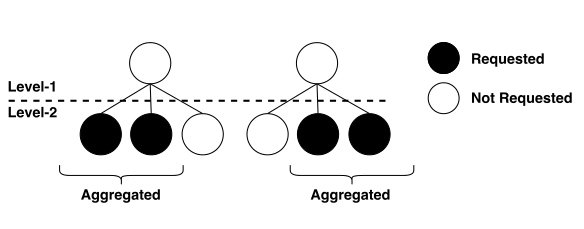
\includegraphics[scale=0.4]{Figs/tree.png}
\caption{A Practical Request Scenario in the Hierarchical Setting}
\label{fig:agg}
\end{figure}

Although the generalized scheme has a two level hierarchy (with each of the $n_1$ parallely executing instances of the basic scheme representing a node in the top level and the actual ciphertext classes representing nodes in the lower level), it avoids the pitfalls of existing hierarchical encryption based schemes \cite{akl1983cryptographic,ateniese2012provably}. In standard tree based hierarchical systems, granting access to the key corresponding to any node implicitly grants access to all the keys in the subtree rooted at that node. This means granting access to a selected set of nodes in a given subtree would blow up the key-size to be the same as the number of nodes. This is avoided in our generalized scheme, since any number of nodes (ciphertext classes) that belong to the same instance may be aggregated into a single key. Figure \ref{fig:agg} summarizes this phenomenon. In the situation depicted, a tree-based hierarchy system would require $4$ decryption keys, while our 
scheme would require only $2$. In this respect, our scheme has similar advantages to that of \cite{chu2014key}.











